% ---------------------------------------------------------
% Vorlage abschlussarbeit.tex
%
% Erstellen: pdflatex, biber, pdflatex, pdflatex
%
% Formatierung für doppelseitigen Druck (dringend empfohlen)
%
% Nutzungshinweis zum Hochschullogo:
%
% Das Logo kann, muss aber nicht auf der Titelseite der Abschlussarbeit
% stehen. Größe und Position des Logos sollen nicht verändert werden; die
% Überlappung mit dem Text ist beabsichtigt. Die Erlaubnis zur Nutzung des
% Logos erstreckt sich nur auf die Abschlussarbeit.
%
% Volker Ahlers, Hochschule Hannover, 2013-2020
% ---------------------------------------------------------

\documentclass[11pt,DIV=12,BCOR=0mm,twoside,openright,headings=normal,%
  numbers=noenddot,headsepline,headinclude]{scrreprt}
\usepackage[automark,headsepline]{scrlayer-scrpage}
\usepackage[utf8]{inputenc}         % UTF8 encoding
\usepackage[T1]{fontenc}
\usepackage{newtxtext,newtxmath}
\usepackage[english]{babel}
\usepackage[fixlanguage]{babelbib}
\usepackage{graphicx}
\usepackage[usenames]{xcolor}
\usepackage{listings}
\usepackage[pdftex]{hyperref}
\usepackage{wallpaper}
\usepackage{physics}
\usepackage{amsmath}
%\usepackage{amssymb}
\usepackage{tikz}
\usepackage{wrapfig}
\usepackage[list=true]{subcaption}
\usepackage[cache=false]{minted}
\usepackage{scrhack}
\usepackage{hhline}
\usepackage{varwidth}
\usepackage{booktabs}
\usepackage{caption}
\usepackage{siunitx}
\usepackage{cases}
\usepackage{needspace}

% You can change the style for code blocks here. See: https://www.overleaf.com/learn/latex/Code_Highlighting_with_minted
\usemintedstyle{rainbow_dash}
\setminted{
linenos,
autogobble,
fontsize=\footnotesize,
breaklines
}

\setcapindent{15pt}

% You can declare your own units here.
\DeclareSIUnit\px{px}
\DeclareSIUnit\atm{atm}
\DeclareSIUnit\AU{AU}

\KOMAoptions{headinclude}
\hypersetup{linkcolor=black,pdfborder=0 0 0}

\tolerance=2000
\emergencystretch 20pt
\frenchspacing

\begin{document}

    \selectlanguage{english}
    \selectbiblanguage{english}

    \thispagestyle{empty}
    \pagenumbering{roman}

    \newlength{\DLROffset}
    \setlength{\DLROffset}{0.05\paperheight}
    \AddToShipoutPicture*{
        \AtPageUpperLeft{
            \raisebox{-\height - \DLROffset}{
                \hspace{\DLROffset}
                
\includegraphics[height=0.13\paperheight]{DLR_Logo.png}
            }
        }
    }

    \newlength{\HsHOffset}
    \setlength{\HsHOffset}{0.05\paperheight}
    \AddToShipoutPicture*{
        \AtPageLowerLeft{
            \parbox[b]{\paperwidth - \HsHOffset}{
                \hfill
                
\includegraphics[height=0.33\paperheight]{hsh-logo}
                \vspace*{\HsHOffset}
            }
        }
    }

    \begin{center}
        \vspace*{4\baselineskip}
        {\sffamily\bfseries\LARGE
        Motion Sickness Reduction for 6-DoF-Navigation in a Virtual Solar System\par}

        \vspace*{4\baselineskip}
        {\Large Moritz Zeumer}

        \vfill
        {\Large Master Thesis}

        \vspace*{4\baselineskip}
        {\Large Hochschule Hannover\\
        Faculty IV -- Business and Computer Science\\
        Course of Studies M.\,Sc.\ Applied Computer Sciences\par}

        \vspace*{4\baselineskip}
        {\Large \today}

        \vspace*{4\baselineskip}
    \end{center}

    \cleardoublepage

    \noindent
    {\sffamily\bfseries Author}

    \vspace*{.5\baselineskip}
    \noindent
    Moritz Zeumer\\
    Matrikelnummer: 1498947\\
    E-Mail: M\_Zeumer@gmx.de

    \vspace*{1\baselineskip}
    \noindent
    {\sffamily\bfseries Examiner}

    \vspace*{.5\baselineskip}
    \noindent
    Prof. Dr. Volker Ahlers\\
    Hochschule Hannover\\
    Faculty IV, Computer Science\\
    Ricklinger Stadtweg 120\\
    30459 Hannover

    \vspace*{1\baselineskip}
    \noindent
    {\sffamily\bfseries Second Examiner}

    \vspace*{.5\baselineskip}
    \noindent
    M. Sc. Simon Schneegans\\
    German Aerospace Center (DLR)\\
    Institute for Software Technology\\
    Software for Space Systems and Interactive Visualization\\
    Lilienthalplatz 7\\
    38108 Braunschweig

    \vfill
    \noindent
    {\sffamily\bfseries Declaration of Authorship}

    \vspace*{.5\baselineskip}
    \noindent
    I hereby declare that this thesis, and the work presented in it are my own and has been generated by me as the result of my own original research.
    I confirm that:

    \begin{enumerate}
        \item Where I have consulted the published work of others, this is always clearly attributed.

        \item Where I have quoted from the work of others, the source is always given.
        Except for such quotations, this thesis is entirely my own work.

        \item I have acknowledged all main sources of help.

        \item Where the thesis is based on work done by myself jointly with others, I have made clear exactly what was done by others and what I have contributed myself.
    \end{enumerate}

    \vspace*{3\baselineskip}
    \noindent
    Hannover, \today\\
    Location and Date\hspace{5cm} Signature

    \tableofcontents

    \cleardoublepage
    \pagenumbering{arabic}

    % Include your chapters here.
    \chapter{Chapter 1}\label{ch:chapter01}

This is a template you can use for your thesis.
In the following some examples will be given how to use the template features.

\section{Some Section}\label{sec:some-section}
This is a section with some text.

\section{Lists}\label{sec:lists}
This is a list:
\begin{itemize}
    \item First item
    \item Second item
    \item Third item
\end{itemize}

\pagebreak

\section{Images}\label{sec:images}

\subsection{Simple Image}\label{subsec:simple-image}

This is an image:
\begin{figure}[h]
    \centering
    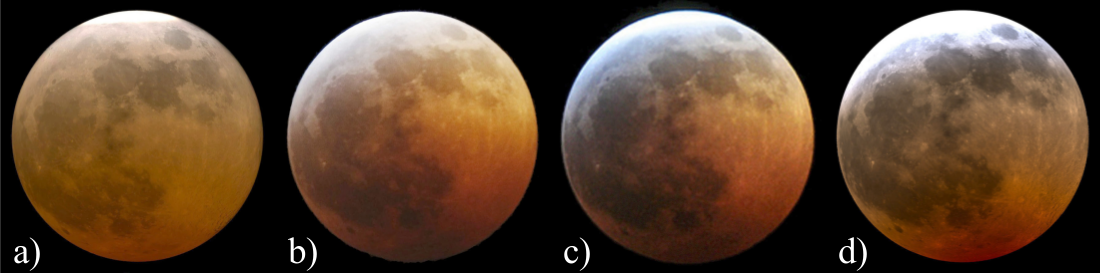
\includegraphics[width=\textwidth]{chapter01/images/Comparison_Yapo_Limberger}
    \caption{This is the image caption. The image is from Limberger et al.~\cite{Limberger2012}.}
    \label{fig:image-example}
\end{figure}


\subsection{Image Comparison}\label{subsec:image-comparison}
\begin{figure}[h]
    \begin{subfigure}[h]{0.45\textwidth}
        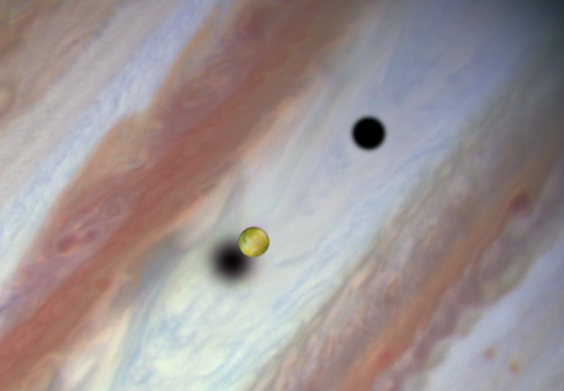
\includegraphics[width=\textwidth]{chapter01/images/HubbleJupiterEclipse2015}
    \end{subfigure}
    \hfill\vrule\hfill
    \begin{subfigure}[h]{0.45\textwidth}
        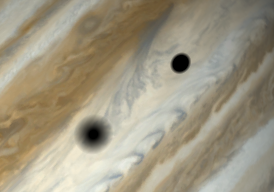
\includegraphics[width=\textwidth]{chapter01/images/CosmoGraphiaEclipseJupiter2015}
    \end{subfigure}

    \caption{Here you can see two images next to another for comparison.}
    \label{fig:image-comparison}
\end{figure}

\section{Citations and References}\label{sec:citations-and-references}
This is a citation: Limberger et al.~\cite{Limberger2012}.

This is a reference to the Appendix~\ref{ch:appendix}.

This is a reference to an image~\ref{fig:image-example}.

Here are some more citations for example purposes at the end of the paper:
\begin{itemize}
    \item Inproceedings~\cite{Yapo2009}
    \item Article~\cite{williams1978}
    \item Website~\cite{celestiaWebsite}
    \item Tech Report~\cite{usStandardAtmosphere}
    \item Master Thesis~\cite{fischer2018}
    \item Book~\cite{bohren1998}
\end{itemize}
    \chapter{Chapter 2}\label{ch:chapter02}

\section{Formulas}\label{sec:formulas}

\begin{wraptable}{o}{0pt}
    \begin{tabular}{|r l|}
        \hline
        \multicolumn{2}{|c|}{\textbf{Symbols}} \\
        \hline
        $I$       & relative brightness \\
        $\Omega_{sun}$  & solid angle of \\
        & the sun \\
        $\Omega_{occ}$  & solid angle of \\
        & intersection \\
        \hline
    \end{tabular}
\end{wraptable}

This is a text that describes a formula.
This formula is for calculating the brightness of light for a single point that is illuminated by the sun and partially occluded by a moon.
This is done by taking the solid angle of the Sun $\Omega_{sun}$ subtracting the solid angle of the occluding moon $\Omega_{occ}$ and normalize the result.
To the right we have a table that describes all the symbols that appear on this page, so people can much more easily see what symbol has which meaning without having to reread the text everytime they want to use the formula.

\begin{equation}
    \label{eq:relative-intensity}
    I = \frac{\Omega_{sun} - \Omega_{occ}}{\Omega_{sun}}.
\end{equation}

\section{Units in Equations}\label{sec:units-in-equations}

\begin{equation}
    \frac{\SI{6371}{\kilo\meter} * \SI{149600000}{\kilo\meter}}{\SI{695510}{\kilo\meter} - \SI{6371}{\kilo\meter}} = \SI{1383000}{\kilo\meter}.\label{eq:equation-with-units}
\end{equation}

\section{Code Blocks}\label{sec:code-blocks}

This templated uses minted for formatting code.
It is required to install the python package Pygments.
You can do this with the following command: pip install Pygments

\subsection{Simple Code Block}\label{subsec:simple-code-block}

Here we can see a code block.
The second argument specifies the language for text highlighting.

\begin{minted}{c}
    // Get the intensity of the eclipse caused by the occluding body for our fragment.
    float eclipseLight = calcEclipse(occludingBody, fragPos);

    // Get the color of the fragment from the bodies texture.
    outputColor = texture(/*...*/);

    // Reduce the brightness of the fragment according to the intensity of the eclipse.
    outputColor = outputColor * eclipseLight;
\end{minted}

\subsection{Imported Code Block from File}\label{subsec:imported-code-block-from-file}

The following line imports code from a text file.
The first argument is the language for highlighting purposes.

\inputminted{c}{chapter02/code/spherical_cap_intersect.glsl}

\subsection{Inline Code}\label{subsec:inline-code}

This is inlined code: \mintinline{c}{float calcEclipse(vec4 occludingBody, vec3 fragmentPosition)}, where the first argument is the language.

\section{Tables}\label{sec:tables}

This is a table:

\begin{center}
    \begin{tabular}{ l r c r}
        \toprule
        \textbf{Body} & \textbf{Semi-major Axis} & \textbf{Observer Placement} & \textbf{Max. Abs. Error} \\
        \midrule
        Mercury & 0.39 AU & surface & 0.0008 \\
        & & 500,000km & 0.0000 \\
        \midrule
        Venus & 0.72 AU & surface & 0.0004 \\
        & & 500,000km & 0.0000 \\
        \midrule
        Earth & 1.00 AU & surface & 0.0003 \\
        & & Moon & 0.0000 \\
        \midrule
        Mars & 1.52 AU & surface & 0.0002 \\
        & & Phobos & 0.0000 \\
        & & Deimos & 0.0000 \\
        \midrule
        Jupiter & 5.20 AU & surface & 0.0000 \\
        & & Io & 0.0000 \\
        & & Callisto & 0.0000 \\
        \bottomrule
    \end{tabular}
    \captionof{table}{This is the table caption.}
    \label{tab:table-example}
\end{center}

    \appendix

    \chapter{Appendix}\label{ch:appendix}

\begin{figure}[h]
    \centering
    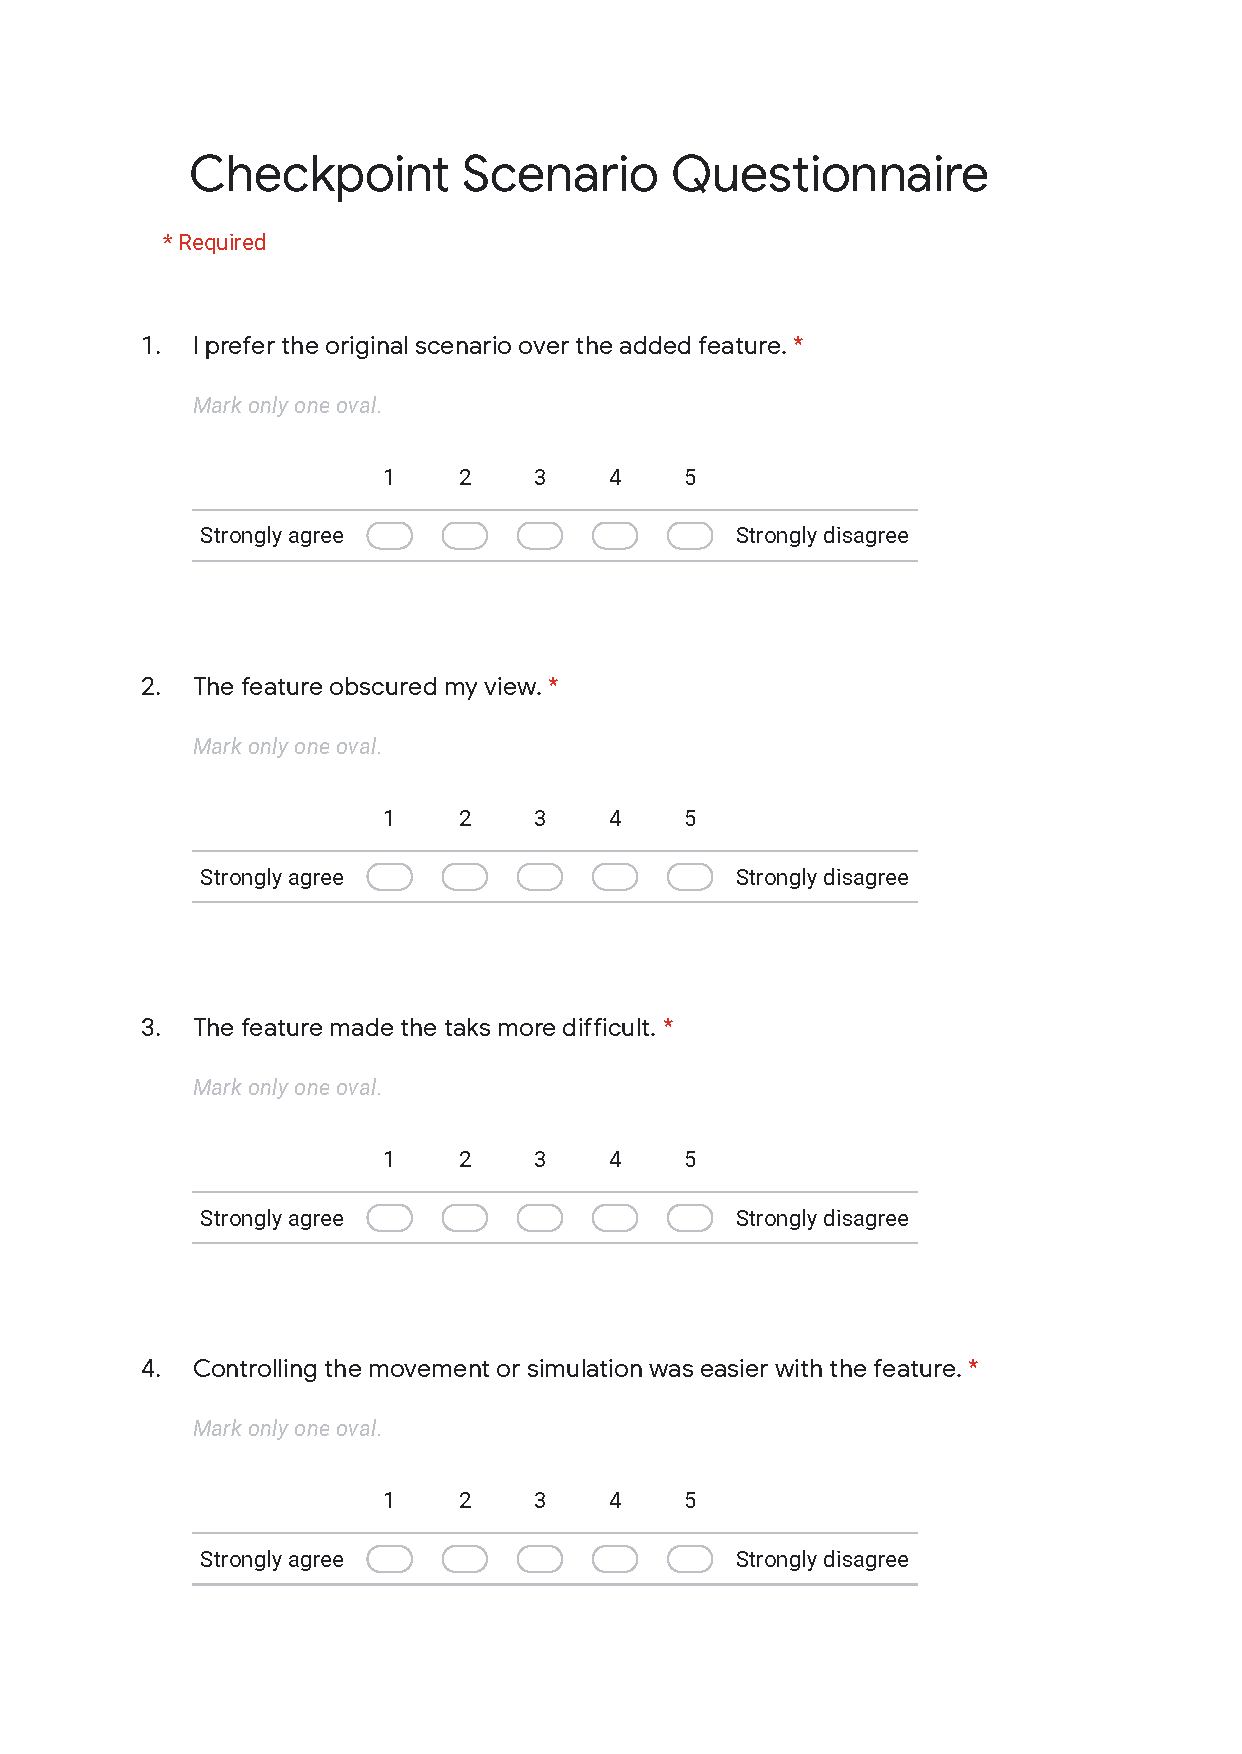
\includegraphics[width=0.8\textwidth]{content/appendix/docs/CheckpointScenarioQuestionnaire}
    \caption{Example questions for the checkpoints scenarios of the user study (page 1).}
    \label{fig:study-checkpoint-questionnaire-1}
\end{figure}

\begin{figure}[h]
    \centering
    \includegraphics[width=0.8\textwidth, page=2]{content/appendix/docs/CheckpointScenarioQuestionnaire}
    \caption{Feedback section for the checkpoints scenarios of the user study (page 2).}
    \label{fig:study-checkpoint-questionnaire-2}
\end{figure}

\begin{figure}[h]
    \centering
    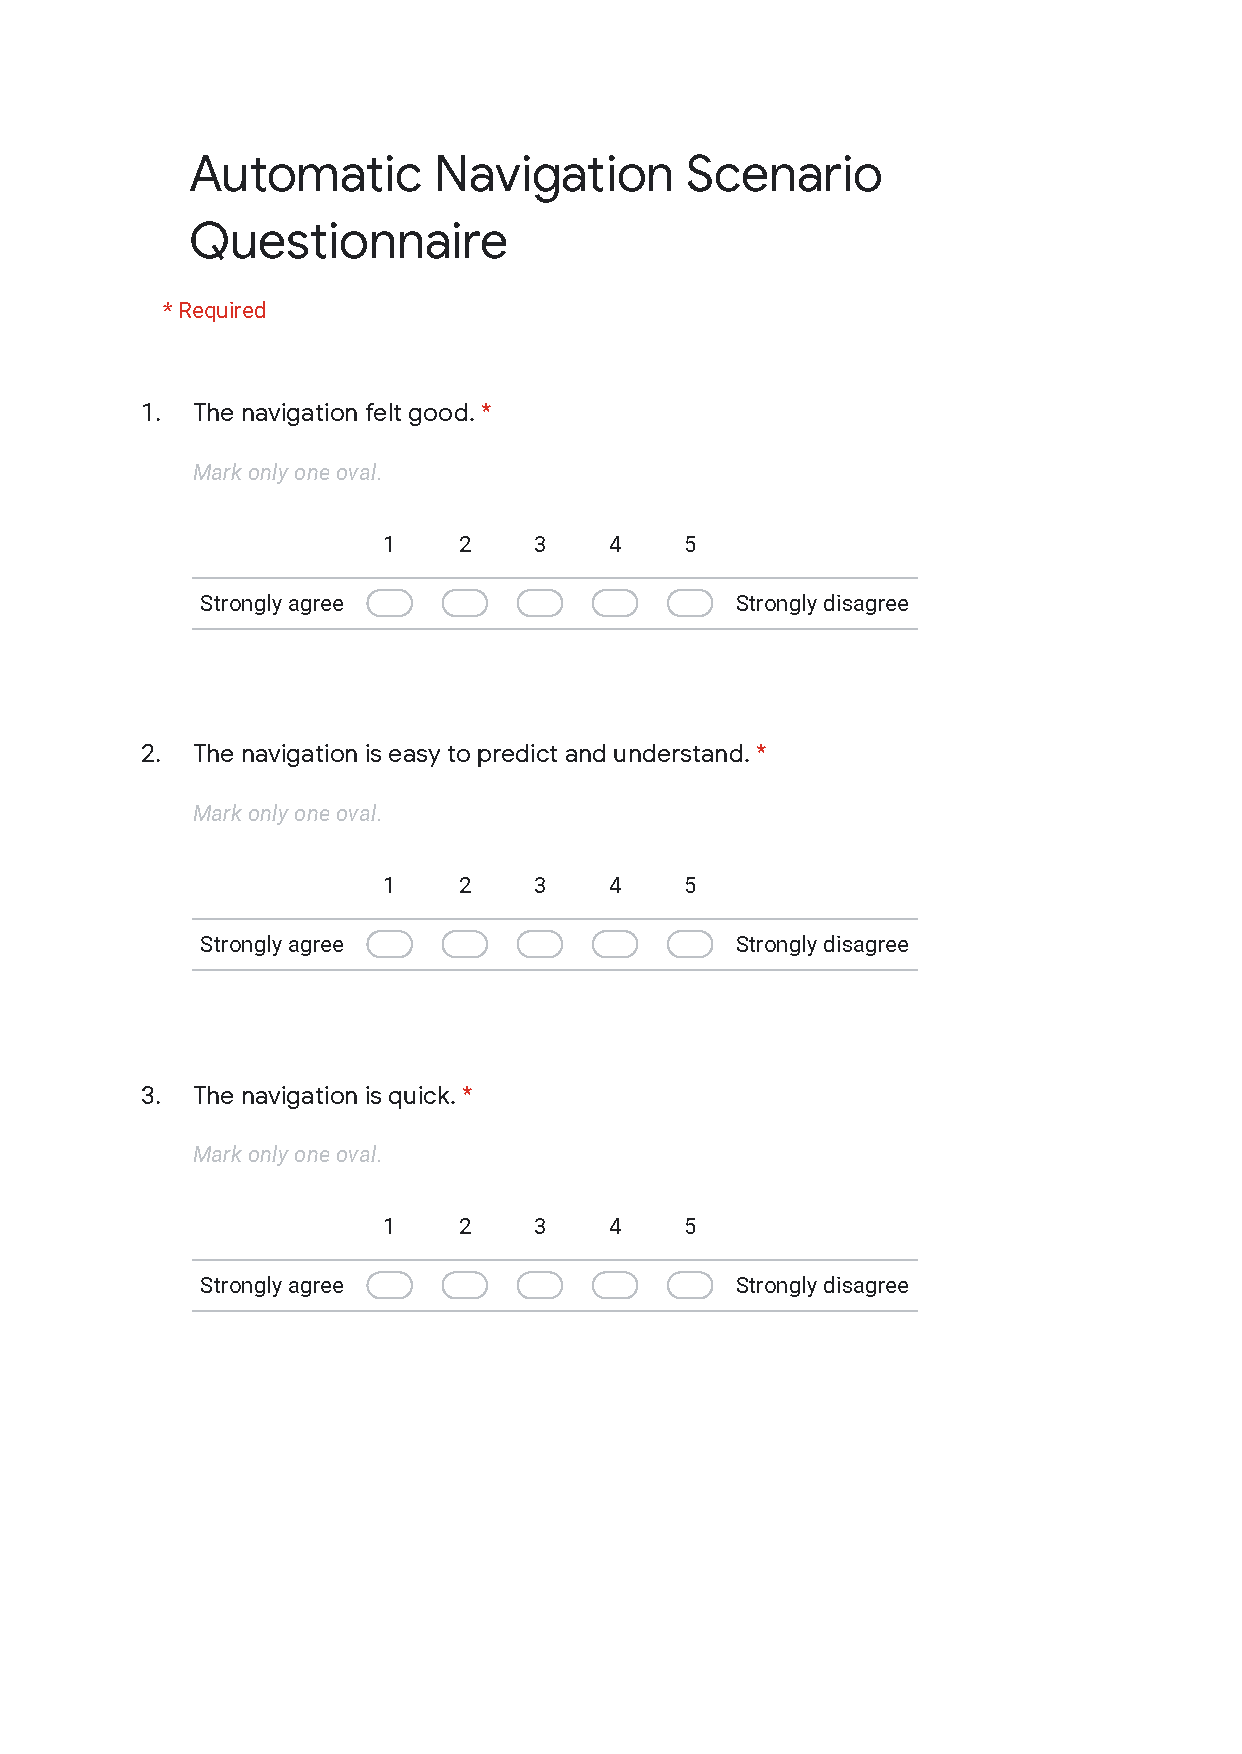
\includegraphics[width=0.8\textwidth]{content/appendix/docs/AutoNavScenarioQuestionnaire}
    \caption{Example questions for the automatic navigation scenarios of the user study (page 1).}
    \label{fig:study-autonav-questionnaire-1}
\end{figure}

\begin{figure}[h]
    \centering
    \includegraphics[width=0.8\textwidth, page=2]{content/appendix/docs/AutoNavScenarioQuestionnaire}
    \caption{Feedback section for the automatic navigation scenarios of the user study (page 2).}
    \label{fig:study-autonav-questionnaire-2}
\end{figure}


    \addcontentsline{toc}{chapter}{Bibliography}
    \renewcommand{\btxfnamespaceshort}{\,}
    \bibliographystyle{bababbrv_unsrt}
    \bibliography{main}

\end{document}
